\documentclass[11pt]{article}
\usepackage{cth_course_template}
\usepackage{times}
\usepackage{url}
\usepackage{latexsym}
\usepackage{graphicx}

\aclfinalcopy % Uncomment this line for the final submission
%\def\aclpaperid{***} %  Enter the acl Paper ID here

\title{This is the Title of the Paper}

\author{First Author \\
  Affiliation / Address line 1 \\
  Affiliation / Address line 2 \\
  Affiliation / Address line 3 \\
  {\tt email@domain} \\\And
  Second Author \\
  Affiliation / Address line 1 \\
  Affiliation / Address line 2 \\
  Affiliation / Address line 3 \\
  {\tt email@domain} \\}

\date{}

\begin{document}
\maketitle
\begin{abstract}
Here goes the abstract.
\end{abstract}

\section{Introduction}
This is the introduction.

\section{A Section}

Start of a section.

\subsection{A Subsection}

Start of a subsection. Table~\ref{table:exampletable} shows an example of a table.

\begin{table}[htb]
\begin{center}
\begin{tabular}{l|c}
%\hline
\hline \bf Column 1 & \bf Column 2\\ \hline
123 & xyz \\
456 & abc %\\
%\hline
\end{tabular}
\end{center}
\caption{Example of a table.}
\label{table:exampletable}
\end{table}

And Figure~\ref{fig:examplefig} shows an example of a figure.

\begin{figure}[htb]
\begin{center}
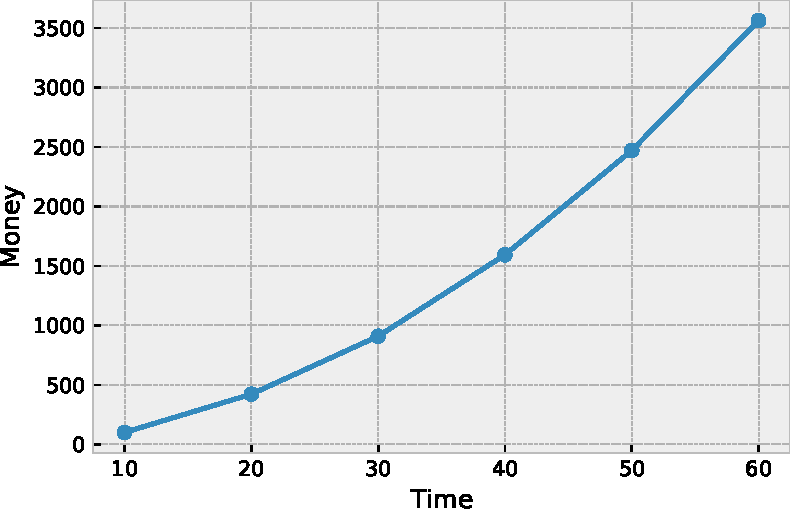
\includegraphics[width=70mm]{example_figure}
\end{center}
\caption{Example of a figure.}
\label{fig:examplefig}
\end{figure}

Citations within the text appear
in parentheses as~\cite{Gusfield:97} or, if the author's name appears in
the text itself, as Gusfield~\shortcite{Gusfield:97}. 
Append lowercase letters to the year in cases of ambiguity.  
Treat double authors as in~\cite{Aho:72}, but write as
 in~\cite{Chandra:81} when more than two authors are involved. Collapse multiple citations as
in~\cite{Gusfield:97,Aho:72}. Also refrain from using full citations as sentence constituents. We
suggest that instead of
\begin{quote}
  ``\cite{Gusfield:97} showed that ...''
\end{quote}
you use
\begin{quote}
``\newcite{Gusfield:97} showed that ...''
\end{quote}

We can also use footnotes.\footnote{This is how a footnote should appear.}

\section{Conclusion}

Our final thoughts are expressed here.

\bibliographystyle{cth_course_template}
\bibliography{template}

\end{document}
